\section{Benchmarks}
We compared the running times of Acme++ and the previous
implementation AcmeML to justify this upgrade. We report the results
in this section.

The comparison is done with regard to the value 1 problem. Since the algorithm
for solving the other problems also relies on computing stabilization monoids
very similar results should be expected if we chose them instead of the value 1
problem.

The probabilistic automata on which the benchmarks were performed, were chosen
in the following way: for each state $s$ we pick a state $t$ with uniform
probability on the set of states and add a transition between $s$ and $t$. After
this we uniformly pick a number $p\in[0,1]$, and for all other states $t'$
different from $t$, we decide whether we will add a transition between $s$ and
$t'$ by flipping a $p$-biased coin.

The results have been plotted in Fig. \ref{bench1}.1. 

If for some sizes of the monoid in the x-axis there is no
corresponding point for the AcmeML implementation, it means that it
either timed out or had a stack overflow.

\begin{figure}[h!]
  %\label{bench1}
  \begin{center}
    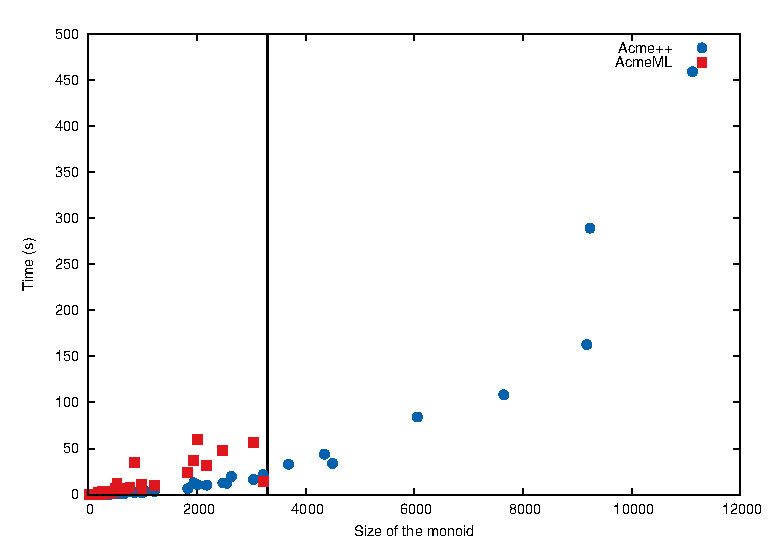
\includegraphics[width=0.45\textwidth]{graph/lines}
    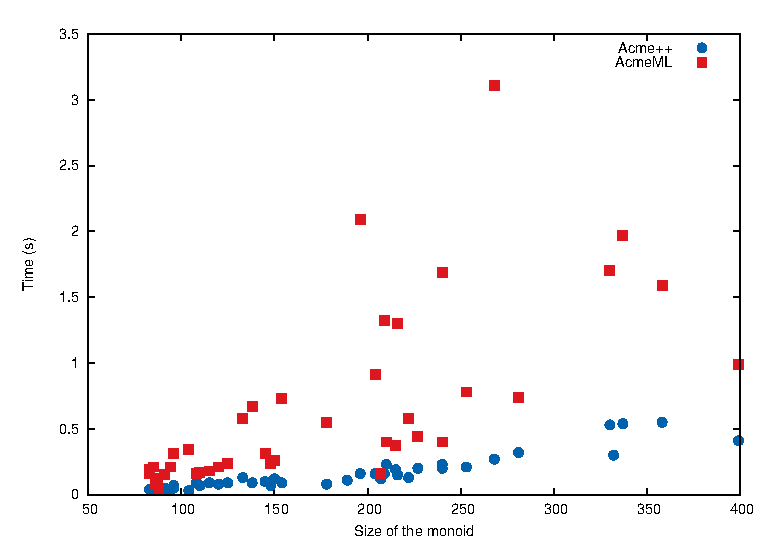
\includegraphics[width=0.45\textwidth]{graph/zoomlines}
    \caption{1)The time it takes for the two implementations to
      calculate the Markov monoids generated by randomly picked
      automata of size 10. 2) The same experiment on automata
      generating smaller Markov monoids}
      \label{bench1}
  \end{center}  
\end{figure}

One can observe that there is a threshold in the size of the Markov
monoid after which AcmeML will not be useful, i.e. it will either take
too much time or have a stack overflow. This threshold is expressed by
the vertical line in Fig. \ref{bench1}.1 (it hovers around 3500 elements).

Even on smaller examples Acme++ outperforms AcmeML by a considerable
factor as seen in Fig. \ref{bench1}.2.

When it comes to the running time for deciding the star-height problem it
completely depends whether the instance is caught by the {\em loop complexity}
heuristic, see Section~\ref{subsec:loop complexity}. In case it is, the running
time is typically a few seconds, otherwise it is too large (i.e. more than the
timeout of 15 minutes for 10 state automata). Consequently a benchmark is not
very illuminating and has been omitted.
%
%\begin{figure}[h!]
%  \label{bench1zoomed}
%  \begin{center}
%    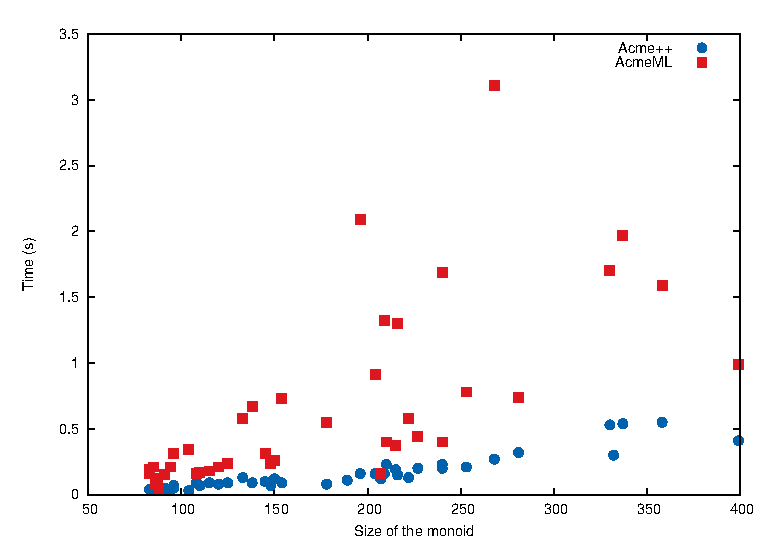
\includegraphics[width=0.5\textwidth]{graph/zoomlines}
%    \caption{The same experiment as in Fig.\ref{bench1} on automata
%      generating smaller Markov monoids}
%  \end{center}  
%\end{figure}
